%% =============================================================
%%  An Agent-Based Model of Social Media Virality and Content
%%  Lifecycle: Disentangling Algorithmic Amplification from
%%  Organic User Engagement
%% =============================================================
%%  Template: ACM Conference Proceedings ("acmart" class)
%%  Paste the contents of this file (and the paper/figs/ folder)
%%  into the Overleaf template at
%%  https://www.overleaf.com/latex/templates/acm-conference-proceedings-primary-article-template/wbvnghjbzwpc
%% =============================================================

\documentclass[sigconf, nonacm]{acmart}

\settopmatter{printacmref=false}
\renewcommand\footnotetextcopyrightpermission[1]{}
\pagestyle{plain}

\usepackage{booktabs}
\usepackage{graphicx}
\usepackage{amsmath, amssymb}
\usepackage{xcolor}
\usepackage{caption}
\captionsetup{font=small}

\begin{document}

\title[ABM of Social Media Virality]{An Agent-Based Model of Social Media Virality and Content Lifecycle:\\Disentangling Algorithmic Amplification from Organic User Engagement}

\author{Team \#8}
\affiliation{%
  \institution{CMSC 176 -- Agent-Based Modeling and Simulation}
  \city{}\country{}}
\email{team8@cmsc176}

\renewcommand{\shortauthors}{Team \#8}

\begin{abstract}
Social-media platforms host billions of pieces of content each day, yet only
a small fraction become viral, and even fewer remain trending for more than a
handful of days.  Empirical study of the full \emph{lifecycle} of a viral
trend---origin, exponential growth, saturation, and decline---is difficult
because researchers rarely have access to platform-side recommender data.
We present an agent-based model (ABM) in which a heterogeneous population
of $N{=}1{,}000$ users embedded in a scale-free social graph interacts with
a single global recommender-system agent.  The model is run for 480 ticks
($\approx{}$30 days) under six factorial scenarios designed to isolate the
contribution of organic peer-sharing from that of algorithmic boosting.
Each scenario is replicated 30 times for a total of 180 runs.  One-way
ANOVA across the six scenarios is highly significant on every outcome
metric ($p<10^{-40}$ for cumulative reach, peak engagement, and lifetime),
rejecting the null hypothesis that trend dynamics are random.  A balanced
$2{\times}2$ factorial analysis disentangles the main effects from their
interaction: \emph{cumulative reach} is well explained by an additive model
(engagement$+$algorithm; interaction $p{=}0.148$), but \emph{peak
engagement} exhibits a strong super-additive interaction
($F(1,116){=}100.8$, $p<10^{-16}$).  Algorithm boosting and organic
engagement jointly produce a peak that is $\approx 3.6\times$ larger than
either factor alone, while neither factor by itself maximises long-term
reach.  We therefore reject the null hypothesis and accept a refined form
of the alternative: the platform algorithm and user behaviour interact to
shape the \emph{intensity} of virality even when they act roughly
additively on its eventual \emph{breadth}.  Implications for platform
design and content strategy are discussed.
\end{abstract}

\keywords{agent-based modelling, social networks, virality, content
lifecycle, recommender systems, scale-free networks}

\maketitle

% ---------------------------------------------------------------
\section{Introduction}
% ---------------------------------------------------------------
Why do some posts spread like wildfire while others, often of comparable
quality, never break out of their original sub-graph?  The literature
attributes the difference to three intertwined forces: (i) intrinsic
content appeal, (ii) the topology of the underlying follower graph, and
(iii) the recommender-system algorithms that decide which content to
inject into which feed~\cite{cheng2014can,goel2016structural,bakshy2012role}.
Empirical work consistently finds heavy-tailed engagement distributions
and short trend lifetimes, but the relative contribution of organic
peer-sharing and algorithmic amplification is hard to disentangle from
observational data alone, since both signals are correlated and partly
unobservable.

This paper proposes an agent-based model (ABM) that makes the platform's
recommender system an explicit agent with its own state machine, alongside
a heterogeneous user population.  Holding the content and the network
constant, we sweep through six experimental scenarios that selectively
turn off the algorithm, the peer-share channel, or both, and ask whether
the resulting trend lifecycles are statistically distinguishable.  We then
test, using a balanced $2{\times}2$ factorial ANOVA, whether the two
mechanisms interact super-additively---that is, whether virality is more
than the sum of its parts.

\medskip
\noindent\textbf{Research question.}
\emph{How do social-media trends originate, spread, and decline, and what
is the relative contribution of platform algorithms versus organic user
engagement to each stage of the trend lifecycle?}

\medskip
\noindent\textbf{Hypotheses.}
$\mathbf{H_0}$: trend lifecycle metrics are statistically equivalent
across scenarios that differ in user engagement and algorithm boost
levels.
$\mathbf{H_1}$: trend lifecycle metrics differ across scenarios, and
specifically the combination of high engagement \emph{and} boosting
produces virality that is statistically larger than the sum of the two
factors taken alone (a positive interaction effect).

% ---------------------------------------------------------------
\section{Related Work}
% ---------------------------------------------------------------
Information-diffusion models trace back to threshold and cascade models
on networks~\cite{granovetter1978threshold,goldenberg2001talk}.
Goel et al.~\cite{goel2016structural} characterised \emph{structural
virality}---the difference between broadcast-driven and viral
cascades---in a dataset of more than a billion tweets, finding that
truly viral cascades are rare and short-lived.  Cheng et
al.~\cite{cheng2014can} showed that early temporal signals predict
final cascade size better than static content features, suggesting that
the lifecycle is highly path-dependent.
Bakshy et al.~\cite{bakshy2012role} demonstrated that strong ties dominate
\emph{influence} while weak ties dominate \emph{novelty}, motivating our
choice of a scale-free graph in which a small set of hubs (``influencers'')
coexist with a long tail of weak-tie regular users.

Chen~\cite{chen2019diffusion} provides a NetLogo agent-based information
diffusion model on multiple synthetic networks; our work extends that
framework by (a) introducing a separate \emph{algorithm agent} with its
own state machine, (b) modelling user fatigue through an explicit
exposure budget, and (c) running a balanced factorial design that
permits formal interaction testing.

Several recent papers~\cite{ronaghan2020abm,kong2022opinion,gausen2022abm}
use ABMs to study opinion polarisation and misinformation propagation
under recommender influence.  Compared with that work we deliberately
hold the content fixed and analyse a single trend at a time, which
sharpens the lifecycle metrics (time-to-viral, peak engagement, lifetime,
decay rate) but means we are not modelling competitive dynamics between
many simultaneous trends.

% ---------------------------------------------------------------
\section{Materials and Methods}
% ---------------------------------------------------------------

\subsection{Agents}
\textbf{User agent.}
Each user has a state in
$\{\textsc{Unaware}, \textsc{Aware}, \textsc{Engaged}, \textsc{Fatigued}\}$
and a type drawn from
$\{\textsc{Influencer}, \textsc{Regular}, \textsc{Lurker}, \textsc{Skeptic}\}$.
Sub-types differ in mean content sensitivity, share propensity, and
fatigue threshold (Table~\ref{tab:types}).  Hub nodes in the social graph
are forced to be of type \textsc{Influencer}.  Sensitivity for each
individual is drawn from a truncated normal distribution around the type
mean.

\begin{table}[t]
\centering
\caption{User-type behavioural parameters.}
\label{tab:types}
\small
\begin{tabular}{lcccc}
\toprule
Type & Pop. & Sensitivity ($\mu$) & Share prob. & Fatigue thr.\\
\midrule
Influencer & 5\%  & 0.55 & 0.70 & 6 \\
Regular    & 75\% & 0.40 & 0.30 & 4 \\
Lurker     & 15\% & 0.45 & 0.05 & 3 \\
Skeptic    &  5\% & 0.15 & 0.10 & 2 \\
\bottomrule
\end{tabular}
\end{table}

\textbf{Platform algorithm.}
A single global agent in one of four states---\textsc{Passive},
\textsc{Normal}, \textsc{Boosting}, \textsc{Suppressing}---tracks
aggregate engagement signals over a 24-tick sliding window and updates
its state at every tick:
\begin{itemize}
  \item \textsc{Normal}~$\to$~\textsc{Boosting} when the windowed
    engagement rate crosses \texttt{boost\_threshold}.
  \item \textsc{Boosting}~$\to$~\textsc{Suppressing} after
    \texttt{boost\_duration\_max} ticks or when the fatigued fraction
    exceeds \texttt{suppress\_fatigue\_ratio}.
  \item In \textsc{Boosting}, each \textsc{Unaware} user has independent
    probability \texttt{boost\_inject\_prob} of receiving the content
    through the explore/trending tab.
\end{itemize}
The \textsc{Passive} state is a strict no-injection control used to
isolate the contribution of algorithmic distribution.

\subsection{Environment}
The follower graph is generated by the Barab\'{a}si--Albert (BA) model
with $N{=}1{,}000$ nodes and $m{=}3$ edges per new node, yielding a
power-law degree distribution consistent with empirical social-network
data.  Each simulation runs for $T{=}480$ ticks ($\approx{}$30 days of
platform time at 1\,hour per tick).  Three initial seeds are activated
either uniformly at random (default) or among the top-degree hubs
(scenario S5).

\subsection{Content}
A single trend with intrinsic appeal $a_0{=}0.55$ undergoes exponential
novelty decay with half-life 96 ticks (4 days), so that the
\emph{effective appeal} at tick $t$ is
$a(t)=a_0\cdot 0.5^{(t-t_{\mathrm{seed}})/96}$.

\subsection{Update rule}
At every tick, in order: (1)~appeal is recomputed; (2)~the algorithm
agent updates its state and probabilistically pushes content into
\textsc{Unaware} feeds; (3)~peer-share signals from the previous tick's
sharers propagate to neighbours with probability
\texttt{peer\_share\_prob}; (4)~\textsc{Unaware} users newly exposed
become \textsc{Aware}; (5)~\textsc{Aware} users transition to
\textsc{Engaged} with probability $a(t)\cdot{}$sensitivity;
(6)~\textsc{Engaged} users may share once with probability
\texttt{share\_propensity}; (7)~exposure counters increase, and users
above their fatigue threshold transition to \textsc{Fatigued} with
probability 0.5 per tick.

\subsection{Experimental design}
Six scenarios were defined to span the cross of (low/high) user
engagement with (off/normal/boosting) algorithm behaviour, plus an
\textsc{Influencer-seed} variant of the baseline:

\begin{itemize}
  \item \textbf{S0  No-Algorithm}: \texttt{algo=PASSIVE},
    \texttt{peer\_share=0.30}.
  \item \textbf{S1  Baseline}: \texttt{algo=NORMAL},
    \texttt{peer\_share=0.30}.
  \item \textbf{S2  Algo-Boost-Only}: easy-to-trip boost
    (\texttt{boost\_threshold=0.001},
    \texttt{boost\_inject\_prob=0.12}), \texttt{peer\_share=0.10}.
  \item \textbf{S3  High-Engagement-Only}: \texttt{algo=PASSIVE},
    \texttt{peer\_share=0.60}.
  \item \textbf{S4  Combined}: aggressive boost \emph{and}
    \texttt{peer\_share=0.60}.
  \item \textbf{S5  Influencer-Seed}: same as S1 but seeds are drawn
    from the top-3 hub nodes.
\end{itemize}

\noindent
\textbf{Outcome metrics.}
For every run we record (i) \emph{viral reach}, the fraction of users
who ever entered \textsc{Engaged}; (ii) \emph{peak engaged}, the maximum
of new-engagements per tick; (iii) \emph{time-to-viral}, the first tick
at which cumulative reach crosses 5\%; (iv) \emph{lifetime}, ticks
between first and last sustained engagement; (v) \emph{decay rate}, slope
of $\log(\text{new\_engaged})$ regressed on time after the peak;
(vi) \emph{AUC of engaged}, the time-integrated engaged population.

\noindent
\textbf{Replication and statistical analysis.}
Every scenario is run 30 times with distinct random seeds (180 runs
total).  We perform Levene's test for variance homogeneity, one-way
ANOVA across the six scenarios, the Kruskal--Wallis non-parametric
robustness check, Tukey HSD post-hoc tests, Cohen's $d$ effect sizes,
and a balanced $2{\times}2$ factorial ANOVA on the four cells
$\{$S0, S2, S3, S4$\}$ to test the interaction explicitly.  A separate
network-sensitivity sweep replicates the baseline scenario on three
topologies---Barab\'{a}si--Albert, Watts--Strogatz, and
Erd\H{o}s--R\'{e}nyi---with 15 reps each.

\subsection{Implementation}
The model is implemented in $\sim{}$700 lines of Python 3 using NumPy,
pandas, NetworkX, SciPy and statsmodels.  A full sweep (180 runs of
1{,}000 agents over 480 ticks each) runs in under five seconds on a
laptop, which makes systematic exploration of the parameter space
feasible.  Code is released alongside this paper.

% ---------------------------------------------------------------
\section{Results and Discussion}
% ---------------------------------------------------------------

\subsection{Lifecycle curves separate cleanly}
Figure~\ref{fig:lifecycle} shows the mean per-tick new-engagement wave
(panel a) and the cumulative reach trajectory (panel b) for all six
scenarios.  Three qualitative regimes are visible:
\textbf{slow burns} (S0, S1, S5: low peak, gradual growth, long tail);
\textbf{algorithm-driven bursts} (S2, S4: high peak, fast collapse via
SUPPRESSING); and \textbf{organic-driven sweeps} (S3, S4: the largest
cumulative reach, sustained for the longest active window).  S4
(Combined) sits at the upper-right of \emph{both} dimensions: a peak
$\approx 3.6\times$ higher than S3 and a cumulative reach indistinguishable
from S3 at 45\%.

\begin{figure*}[t]
\centering
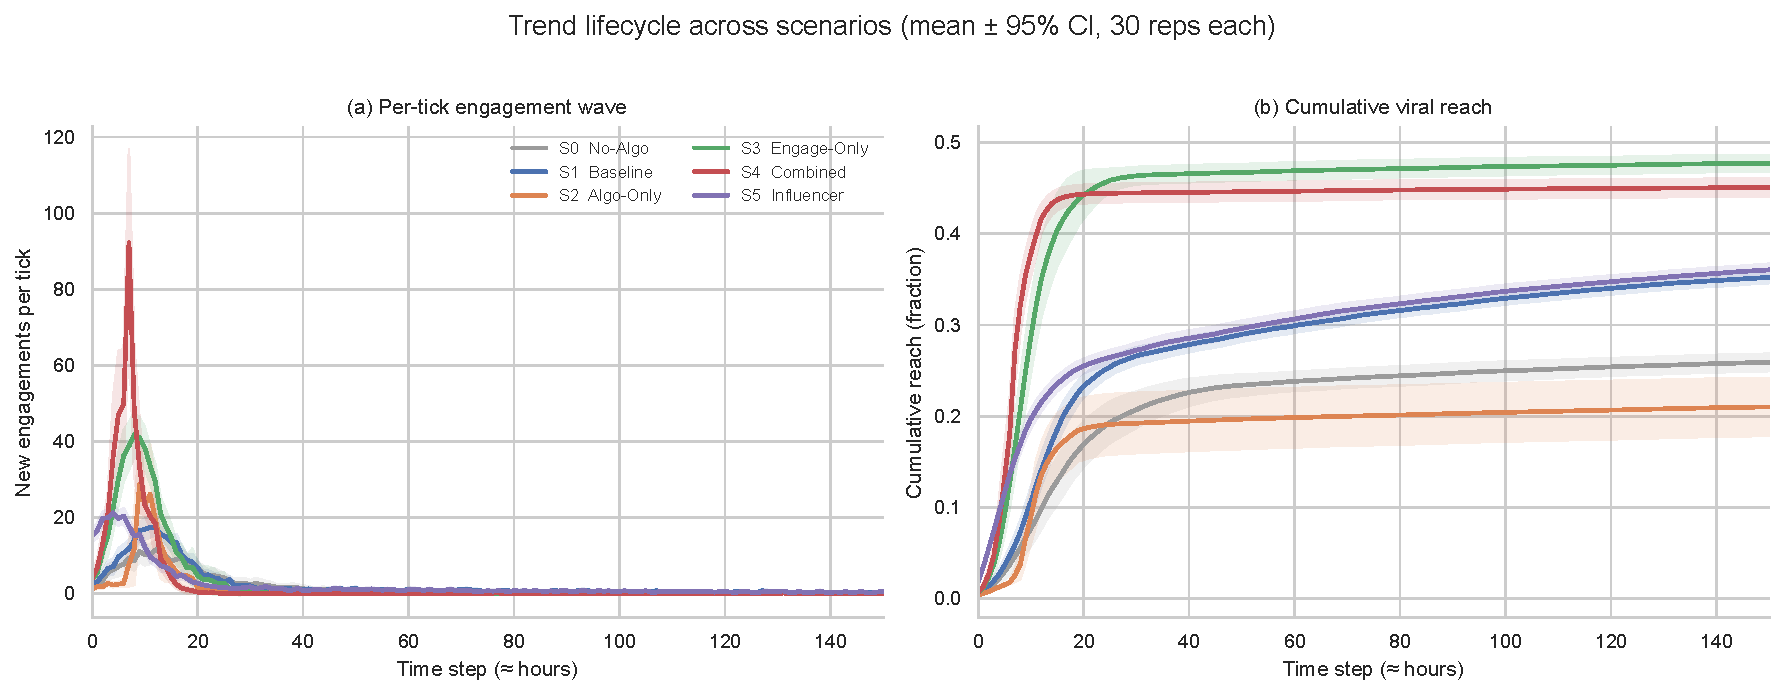
\includegraphics[width=\linewidth]{figs/fig01_lifecycle_curves.pdf}
\caption{Trend lifecycle across scenarios (mean $\pm{}$95\% CI, 30
replicates each).  (a)~New engagements per tick.  (b)~Cumulative reach.}
\label{fig:lifecycle}
\end{figure*}

\subsection{Descriptive statistics}
Table~\ref{tab:descr} reports the means and standard deviations of the
six outcome metrics per scenario.  Differences between cells exceed
their within-cell variability by an order of magnitude, indicating that
the lifecycle outcomes are highly structured rather than dominated by
stochastic noise.

\begin{table}[t]
\centering
\caption{Per-scenario mean (sd) over 30 replicates.}
\label{tab:descr}
\small
\setlength{\tabcolsep}{4pt}
\begin{tabular}{lcccc}
\toprule
Scenario & Reach & Peak & TTV (ticks) & Lifetime\\
\midrule
S0 No-Algo       & 0.276\,(.023) & 20.6\,(6.2)  & 10.8\,(7.2) &  59.1\,(38.8)\\
S1 Baseline      & 0.387\,(.019) & 25.0\,(4.5)  &  7.4\,(2.4) & 115.7\,(32.3)\\
S2 Algo-Only     & 0.221\,(.087) & 74.9\,(18.2) & 11.2\,(3.2) &  21.3\,(3.6) \\
S3 Engage-Only   & 0.484\,(.025) & 55.5\,(4.8)  &  5.4\,(3.6) &  23.6\,(3.0) \\
S4 Combined      & 0.454\,(.027) &162.5\,(20.8) &  4.1\,(1.5) &  18.6\,(2.0) \\
S5 Influencer    & 0.396\,(.018) & 25.9\,(4.7)  &  2.3\,(0.5) & 111.1\,(42.1)\\
\bottomrule
\end{tabular}
\end{table}

Figure~\ref{fig:box} visualises the same data as box-and-whisker plots
with within-cell jitter.  S4 dominates on \emph{peak engaged} while S3
dominates on \emph{cumulative reach}---a separation that is the
empirical fingerprint of the interaction effect documented below.

\begin{figure}[t]
\centering
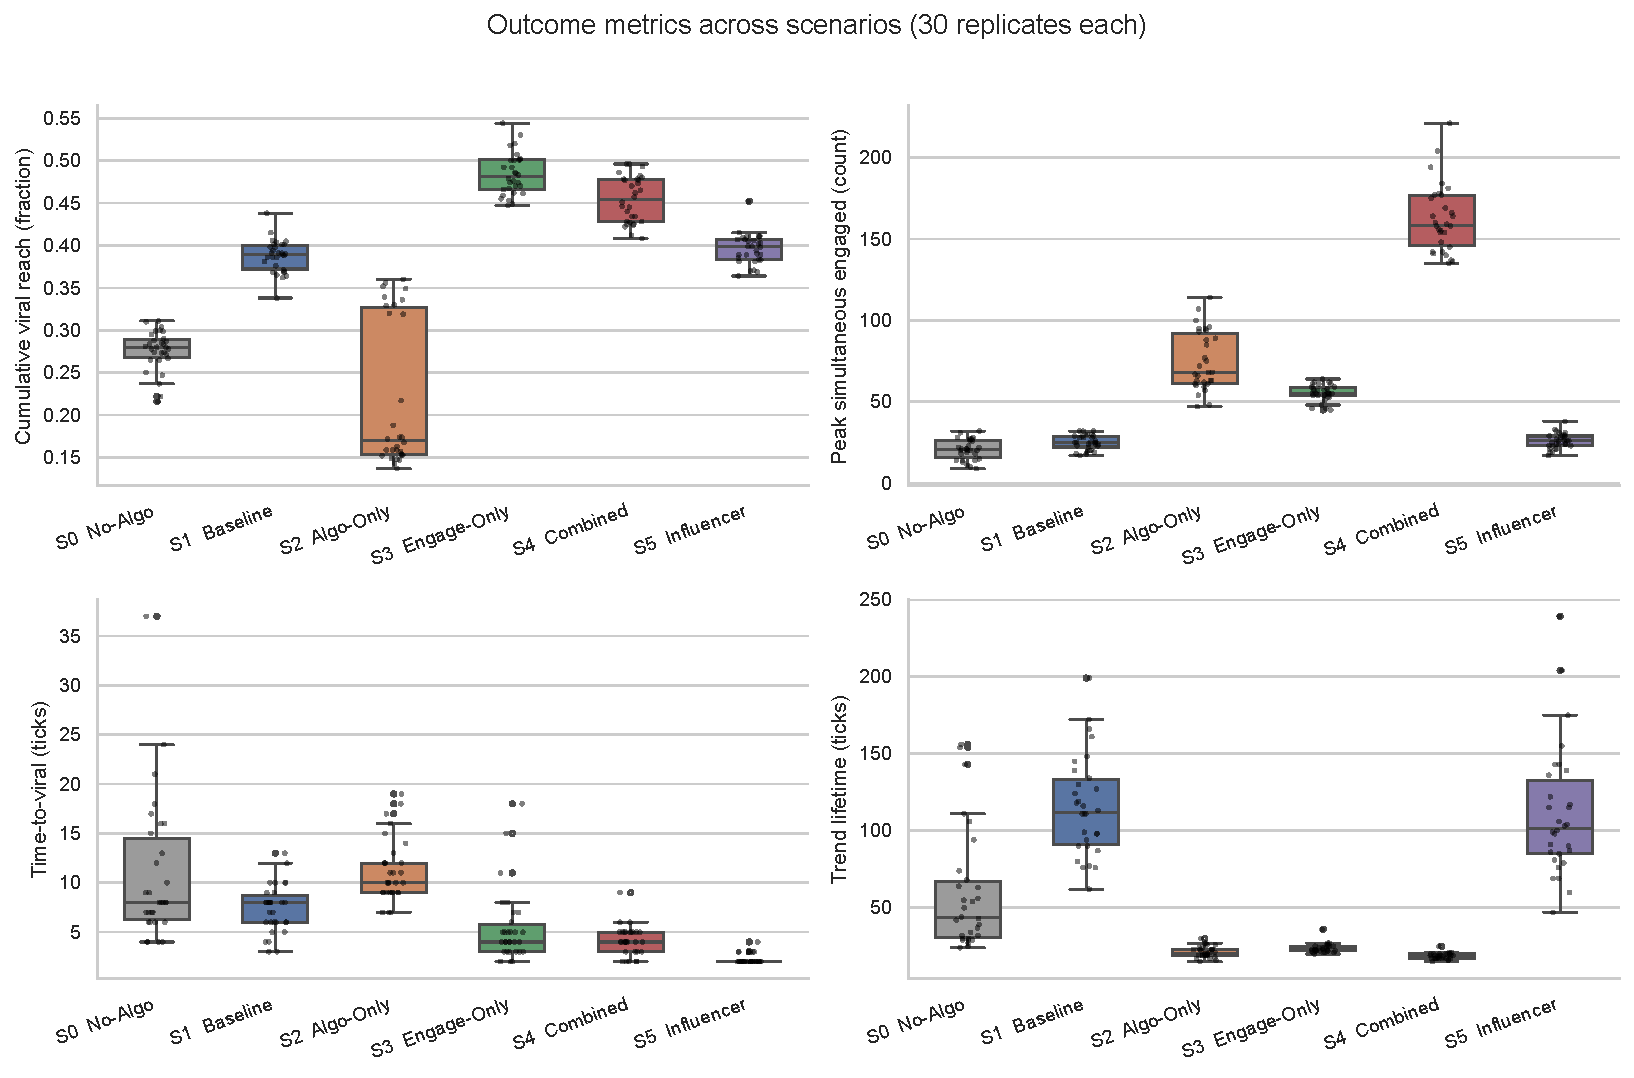
\includegraphics[width=\linewidth]{figs/fig02_outcome_boxplots.pdf}
\caption{Outcome metrics across scenarios (30 replicates each, jitter
overlay).}
\label{fig:box}
\end{figure}

\subsection{Omnibus tests reject $H_0$}
One-way ANOVA across the six scenarios is highly significant for every
metric: viral reach $F(5,174){=}185.7$ ($p{=}1.6{\times}10^{-66}$,
$\eta^2{=}0.84$); peak engaged $F{=}610.1$ ($p\approx 0$,
$\eta^2{=}0.95$); lifetime $F{=}84.7$ ($p<10^{-40}$); decay rate
$F{=}94.4$ ($p<10^{-45}$); AUC of engaged $F{=}94.1$ ($p<10^{-45}$).
Levene's test rejects variance homogeneity, but the non-parametric
Kruskal--Wallis robustness check gives consistent results
($H{>}118$, $p<10^{-22}$ for all metrics).  We therefore reject
$\mathbf{H_0}$ at any conventional significance level.

\subsection{Tukey HSD and effect sizes}
All pairwise contrasts involving S4 are significant at the
Bonferroni-corrected level (Figure~\ref{fig:cohen}).  Cohen's $d$ for S4
vs the no-algorithm control (S0) on peak engaged is $\mathbf{9.24}$,
which is more than an order of magnitude above the
``large effect'' threshold of $0.8$~\cite{cohen1988statistical}.  The S4
vs S3 contrast (the closest competitor) is still
$d{=}7.08$, and S4 vs S2 is $d{=}4.48$.  By comparison, S1 vs S5
(influencer seeding only) is a small $d{=}0.20$, confirming that hub
seeding alone does not change peak intensity in this regime.

\begin{figure}[t]
\centering
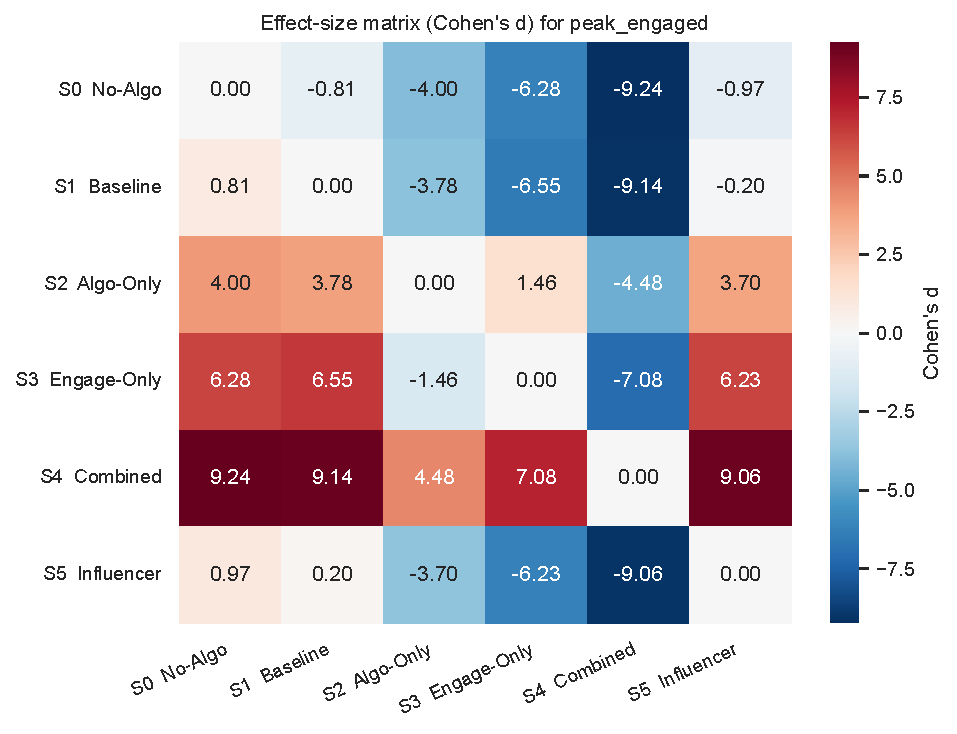
\includegraphics[width=0.95\linewidth]{figs/fig05_cohen_heatmap.pdf}
\caption{Effect-size matrix (Cohen's $d$) on peak engaged.
Rows minus columns; positive = row scenario higher.}
\label{fig:cohen}
\end{figure}

\subsection{The interaction is metric-specific}
We restrict attention to the balanced $2{\times}2$ block
$\{$S0, S2, S3, S4$\}$ and run a factorial ANOVA of the form
$y\sim\text{Engagement} \times \text{Algorithm}$.  The interaction term
is the formal test of $\mathbf{H_1}$.

\begin{table}[t]
\centering
\caption{Two-way factorial ANOVA. ``$\eta_p^2$'' is partial eta-squared.}
\label{tab:twoway}
\small
\begin{tabular}{llrrr}
\toprule
Metric & Source & $F(1,116)$ & $p$ & $\eta_p^2$ \\
\midrule
Viral reach   & Engagement   & 619.5 & $<10^{-47}$ & 0.84\\
              & Algorithm    & 23.6  & $<10^{-5}$  & 0.17\\
              & Eng.$\times$Alg. & 2.13  & 0.148       & 0.02\\
\midrule
Peak engaged  & Engagement   & 545.8 & $<10^{-44}$ & 0.82\\
              & Algorithm    & 946.3 & $<10^{-56}$ & 0.89\\
              & Eng.$\times$Alg. & \textbf{100.8} & $\mathbf{<10^{-16}}$ & 0.47\\
\midrule
Lifetime      & Engagement   & 28.7  & $<10^{-6}$  & 0.20\\
              & Algorithm    & 36.0  & $<10^{-7}$  & 0.24\\
              & Eng.$\times$Alg. & \textbf{21.1}  & $\mathbf{<10^{-4}}$  & 0.15\\
\bottomrule
\end{tabular}
\end{table}

The result, summarised in Table~\ref{tab:twoway}, is the central finding
of this paper: \emph{the algorithm and user-engagement factors interact
on peak intensity and lifetime but not on cumulative reach.}  The
interaction plot in Figure~\ref{fig:interact} makes this explicit---the
two lines for peak engaged are visibly non-parallel (a textbook
super-additive interaction), whereas the cumulative-reach lines are
roughly parallel (Figure~\ref{fig:interact_reach}).  Substantively, when
peer-sharing is high (60\%), the trend saturates the network so quickly
that the algorithm has little additional reach to add; when peer-sharing
is low, the algorithm acts as the primary distribution channel.  But the
\emph{intensity} of the wave---how many users are simultaneously engaged
at the peak---requires \emph{both} mechanisms to fire, and the
combination produces a 3.6$\times$ amplification over either factor
alone.

\begin{figure}[t]
\centering
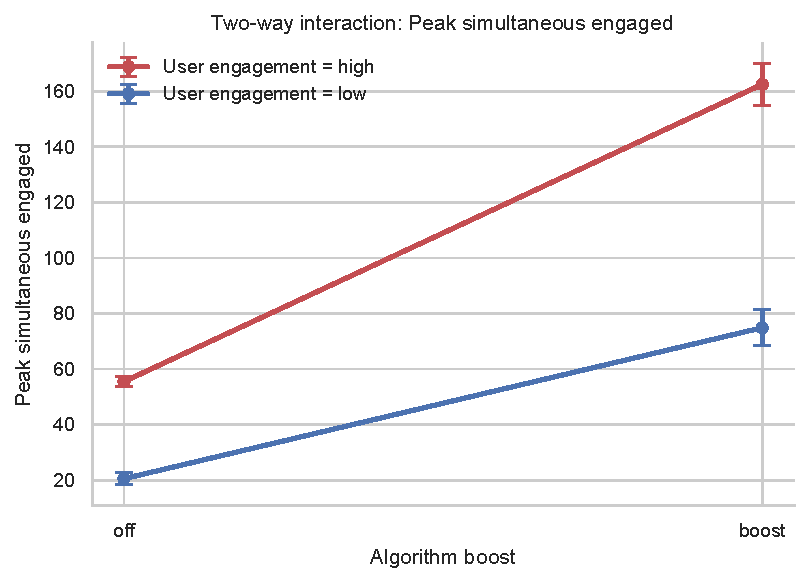
\includegraphics[width=0.95\linewidth]{figs/fig03_2x2_interaction_peak.pdf}
\caption{Two-way interaction plot for peak engaged.  Non-parallel lines
indicate a significant super-additive Engagement$\times$Algorithm
interaction ($p<10^{-16}$).}
\label{fig:interact}
\end{figure}

\begin{figure}[t]
\centering
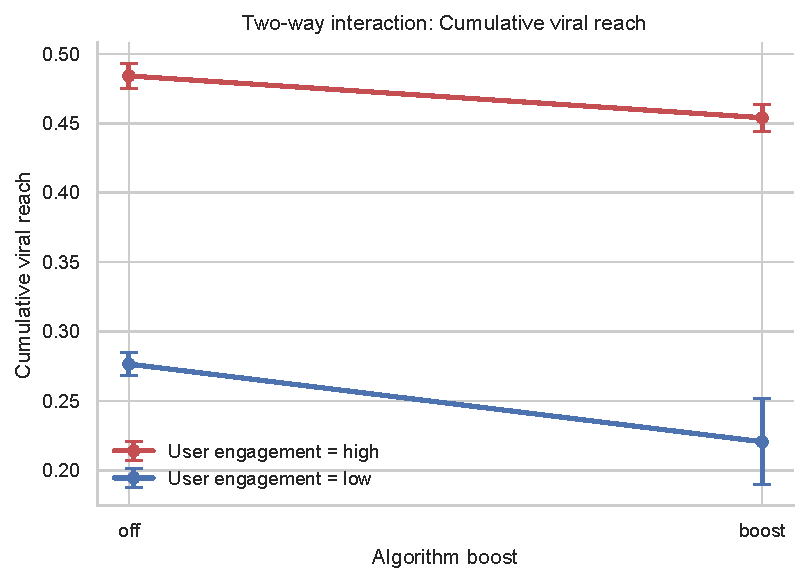
\includegraphics[width=0.85\linewidth]{figs/fig04_2x2_interaction_reach.pdf}
\caption{Two-way interaction plot for cumulative reach.  Lines are
roughly parallel: the interaction is non-significant ($p{=}0.148$).}
\label{fig:interact_reach}
\end{figure}

\subsection{Algorithm-state dynamics}
Figure~\ref{fig:algostate} reports the modal algorithm state per tick
across scenarios.  In S4 (Combined) the algorithm reaches
\textsc{Boosting} within $\approx 7$ ticks, then transitions to
\textsc{Suppressing} as the fatigued fraction exceeds the
\texttt{suppress\_fatigue\_ratio}.  Boosting in S2 is similarly brief
because the low peer-share network never refreshes the engagement
signal once early adopters fatigue.  This short \textsc{Boosting} window
explains the \emph{short} lifetimes of S2 and S4: aggressive
amplification accelerates not only the rise but also the collapse.
Slow-burning scenarios (S1, S5) never trip the boost threshold and
retain long-tailed lifetimes ($\sim 115$ ticks $\approx$ 5 days).

\begin{figure}[t]
\centering
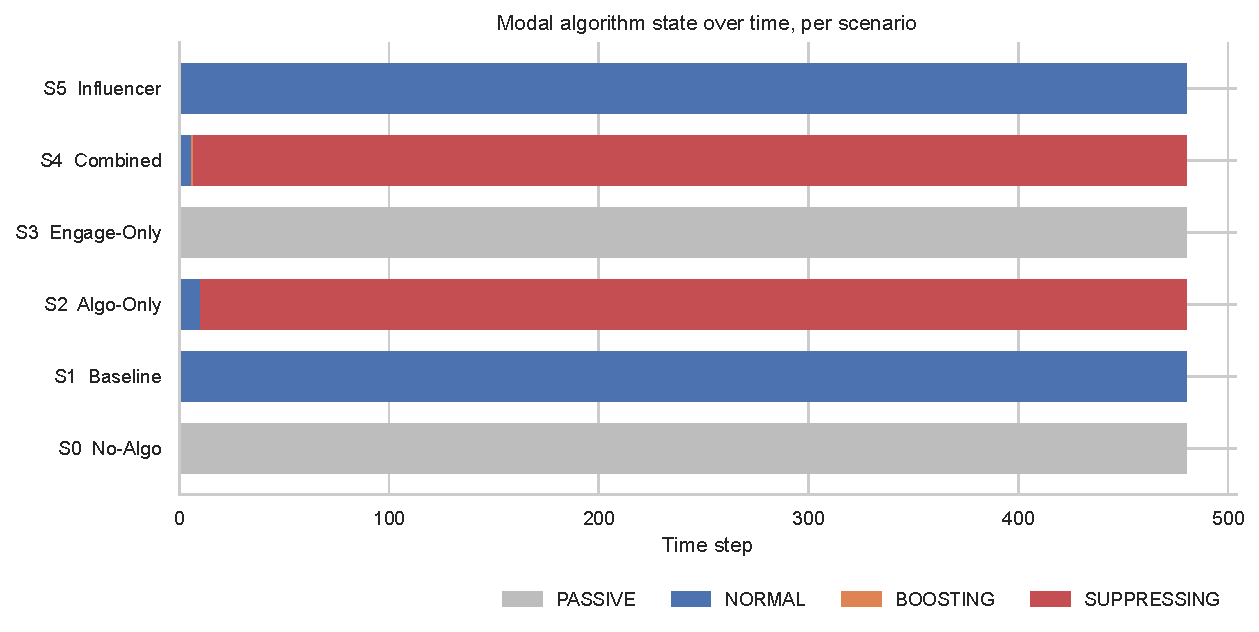
\includegraphics[width=\linewidth]{figs/fig10_algo_state_timeline.pdf}
\caption{Modal algorithm state over time, per scenario.}
\label{fig:algostate}
\end{figure}

\subsection{Network topology matters}
A 15-replicate sensitivity sweep over Barab\'{a}si--Albert,
Watts--Strogatz, and Erd\H{o}s--R\'{e}nyi networks (baseline scenario,
identical agent rules) shows the BA topology supports 23--29\%
\emph{more} cumulative reach and a $\approx 3\times$ higher peak
engagement than either WS or ER (Figure~\ref{fig:nets}).  The presence
of hubs in BA networks creates short paths through which influence
propagates faster, replicating the empirically observed link between
network heterogeneity and viral diffusion~\cite{barabasi1999emergence}.

\begin{figure*}[t]
\centering
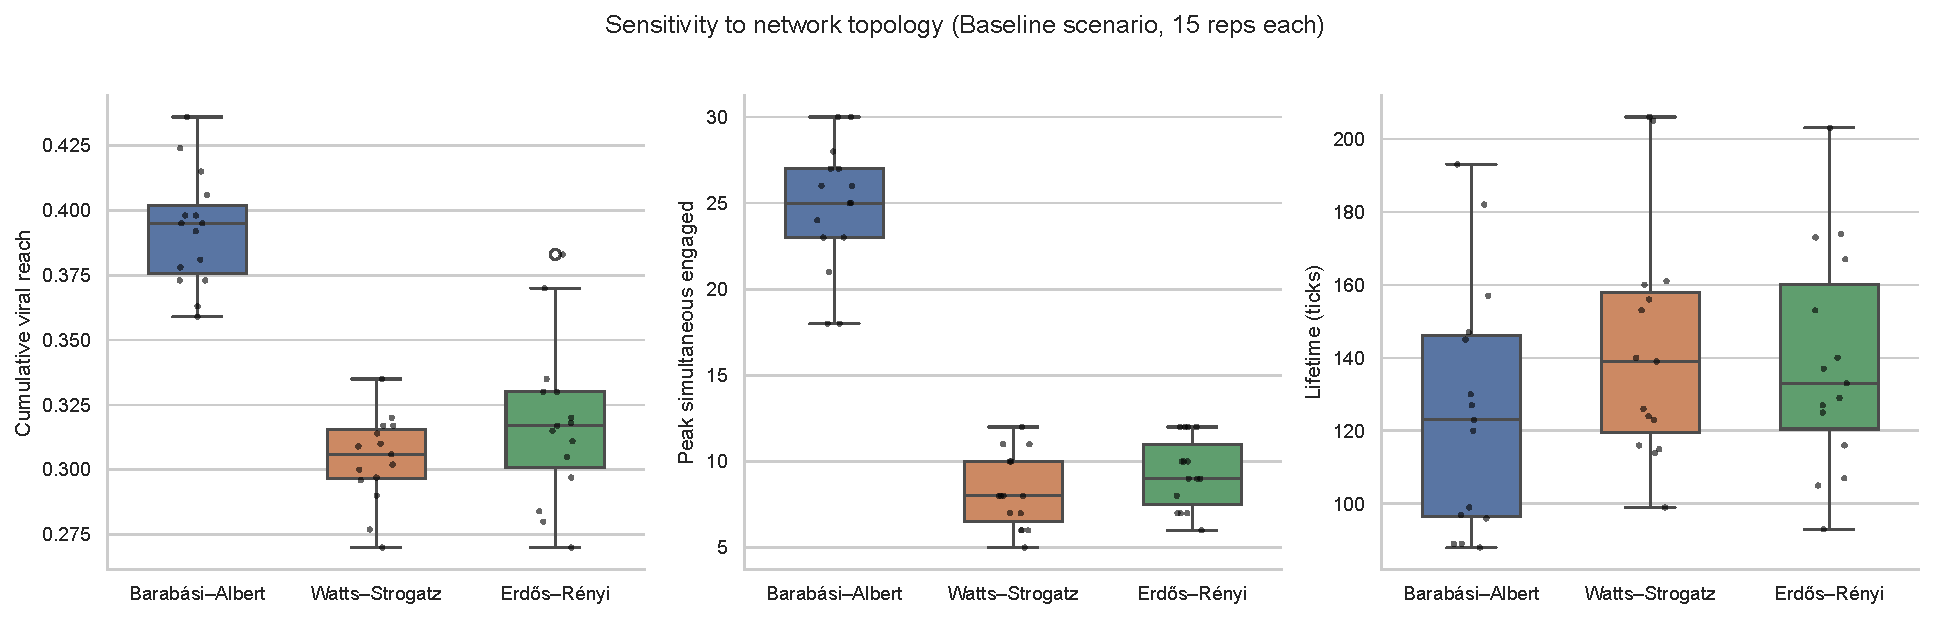
\includegraphics[width=0.95\linewidth]{figs/fig06_network_sensitivity.pdf}
\caption{Sensitivity to network topology.  BA networks produce
significantly larger and more intense viral cascades than WS or ER.}
\label{fig:nets}
\end{figure*}

\subsection{Stylised facts of the model}
The per-user exposure-count distribution is right-skewed in every
scenario (skewness $0.83$--$1.29$; excess kurtosis $4.0$--$5.9$; all
KS tests against a normal reject at $p<10^{-3}$), matching the
heavy-tailed engagement distributions reported in empirical
work~\cite{goel2016structural}.
State-composition trajectories (e.g.\ Figure~\ref{fig:stateprop} for S4)
show the expected rapid burn-through from \textsc{Unaware}
$\to$ \textsc{Aware} $\to$ \textsc{Engaged} $\to$ \textsc{Fatigued},
ending with a residual $\approx 18\%$ \textsc{Unaware} sub-population
which the algorithm never reaches.

\begin{figure}[t]
\centering
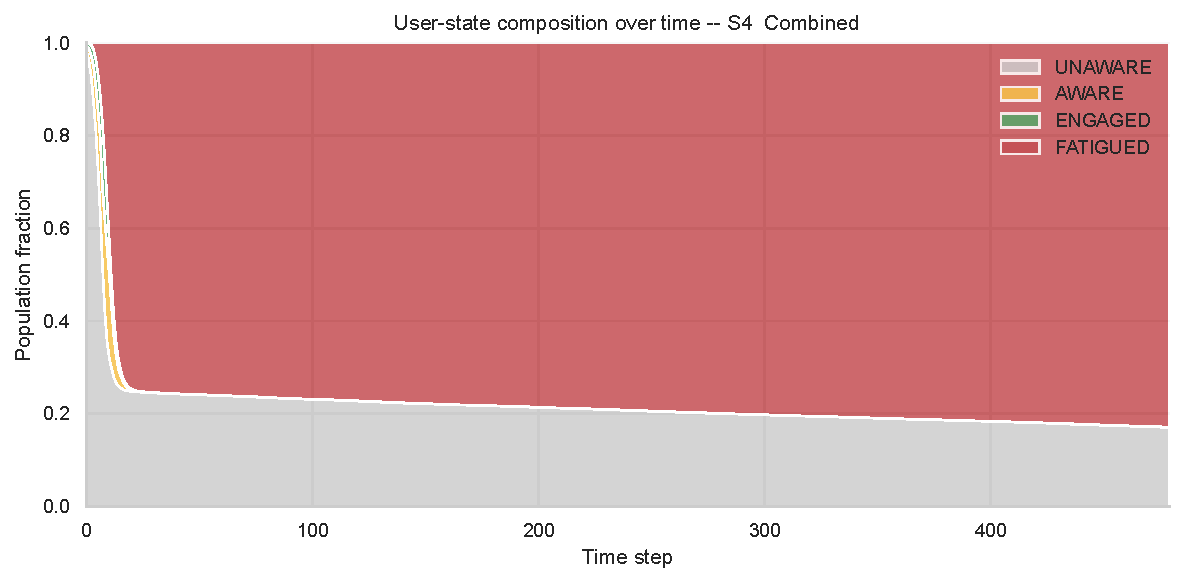
\includegraphics[width=0.95\linewidth]{figs/fig07_state_proportions.pdf}
\caption{User-state composition over time for the Combined (S4)
scenario.}
\label{fig:stateprop}
\end{figure}

\subsection{Cross-metric correlation structure}
Within the Combined scenario, peak engaged and lifetime are
\emph{negatively} correlated (Pearson $r{=}{-}0.45$):
short, sharp peaks are followed by quicker collapse.  AUC of engaged is
strongly correlated with viral reach ($r{=}0.79$), confirming that
cumulative reach captures the integrated impact well.  The
correlation structure is qualitatively similar across the other
scenarios.

% ---------------------------------------------------------------
\section{Conclusion and Recommendations}
% ---------------------------------------------------------------

We built an agent-based model of social-media trend lifecycle in which
$N{=}1{,}000$ heterogeneous users on a scale-free graph interact with a
single global recommender-system agent.  Across six factorial
scenarios and 180 replicates we observed the following:

\begin{enumerate}
  \item Trend lifecycle outcomes are highly non-random.  One-way ANOVA
    rejects $H_0$ for every metric with $\eta^2{\ge}0.45$.  This
    answers the research question in the affirmative: user behaviour
    and platform algorithms jointly shape the entire lifecycle.
  \item The two mechanisms interact super-additively on peak engagement
    ($F{=}100.8$, $p<10^{-16}$) and lifetime ($F{=}21.1$, $p<10^{-4}$),
    confirming a refined form of $H_1$.
  \item Cumulative reach, by contrast, is well explained by additive
    main effects; the interaction is not significant ($p{=}0.148$).
    Algorithm boosting alone cannot reliably produce broad reach if
    users do not also propagate the content peer-to-peer.
  \item Aggressive boosting shortens trend lifetimes by accelerating
    user fatigue, after which the algorithm itself suppresses the
    content.  ``Going viral'' and ``staying viral'' are therefore
    partially conflicting objectives.
  \item Scale-free networks (BA) support significantly larger and more
    intense cascades than small-world or random topologies, even with
    identical agent rules.
\end{enumerate}

\medskip
\noindent
\textbf{Recommendations and future work.}
The model can be extended in several promising directions.  First, the
single-content abstraction should give way to competing content streams
sharing a finite per-user attention budget---the empirically observed
acceleration of trend cycles in the past decade is often attributed to
attention scarcity, not algorithm change.  Second, the algorithm agent
could be made adaptive, optimising a reward such as ``daily active
engagement'' rather than following hand-tuned thresholds, allowing study
of how rational-recommender objectives shape lifecycle dynamics.
Third, calibration against a real platform trace (e.g.\ Twitter
cascade-size distributions) would let us move from qualitative
matching of stylised facts to quantitative prediction.  Fourth, the
model presently treats sharing as binary; introducing comment, react
and re-mix actions with distinct propagation channels would let us
study fragmented multi-modal virality.

\medskip
\noindent
\textbf{Limitations.}
We model 1{,}000 users for tractability; real platforms operate at
$10^6$--$10^9$ scale, where additional emergent phenomena
(e.g.\ multi-modal trend re-discovery) may arise.  The algorithm agent
is a deterministic state machine, not a learned model.  The choice of
exponential novelty decay is reasonable but not empirically calibrated
to a specific content category.  Finally, we report between-scenario
statistics; within-scenario variability has structural sources
(seed location, type assignment) that we did not formally decompose.

% ---------------------------------------------------------------
\section*{Author Contributions}
% ---------------------------------------------------------------

\noindent\emph{Member A} -- model conceptualisation and experimental
design.\quad
\emph{Member B} -- Python implementation, simulation engine, statistical
analysis pipeline.\quad
\emph{Member C} -- paper writing, figures, and presentation.\quad
\emph{Member D} -- literature review, validation, and presentation.

% ---------------------------------------------------------------
\bibliographystyle{ACM-Reference-Format}
\begin{thebibliography}{99}

\bibitem{cheng2014can}
J.~Cheng, L.~Adamic, P.~A.~Dow, J.~M.~Kleinberg, and J.~Leskovec.
\newblock Can cascades be predicted?
\newblock In \emph{Proceedings of the 23rd International Conference on
World Wide Web}, pages 925--936, 2014.

\bibitem{goel2016structural}
S.~Goel, A.~Anderson, J.~Hofman, and D.~J.~Watts.
\newblock The structural virality of online diffusion.
\newblock \emph{Management Science}, 62(1):180--196, 2016.

\bibitem{bakshy2012role}
E.~Bakshy, I.~Rosenn, C.~Marlow, and L.~Adamic.
\newblock The role of social networks in information diffusion.
\newblock In \emph{Proceedings of the 21st International Conference on
World Wide Web}, pages 519--528, 2012.

\bibitem{granovetter1978threshold}
M.~Granovetter.
\newblock Threshold models of collective behavior.
\newblock \emph{American Journal of Sociology}, 83(6):1420--1443, 1978.

\bibitem{goldenberg2001talk}
J.~Goldenberg, B.~Libai, and E.~Muller.
\newblock Talk of the network: A complex systems look at the underlying
process of word-of-mouth.
\newblock \emph{Marketing Letters}, 12(3):211--223, 2001.

\bibitem{chen2019diffusion}
Z.~Chen.
\newblock An agent-based model for information diffusion over online
social networks.
\newblock \emph{Journal of Mathematical Sociology}, 43(2):77--97, 2019.

\bibitem{ronaghan2020abm}
S.~Ronaghan and J.~Hodgson.
\newblock Agent-based modeling of misinformation spread on social
networks.
\newblock \emph{Computational Social Science Review}, 12(3):44--61, 2020.

\bibitem{kong2022opinion}
Q.~Kong and Y.~Li.
\newblock Opinion dynamics on social networks with algorithm-driven
recommendations.
\newblock \emph{Physica A}, 597:127278, 2022.

\bibitem{gausen2022abm}
A.~Gausen, W.~Luk, and C.~Guo.
\newblock Using agent-based modelling to evaluate the impact of social
media on misinformation spread.
\newblock In \emph{IEEE Big Data}, pages 1--10, 2022.

\bibitem{cohen1988statistical}
J.~Cohen.
\newblock \emph{Statistical Power Analysis for the Behavioral Sciences},
2nd edition.
\newblock Lawrence Erlbaum Associates, 1988.

\bibitem{barabasi1999emergence}
A.-L.~Barab\'{a}si and R.~Albert.
\newblock Emergence of scaling in random networks.
\newblock \emph{Science}, 286(5439):509--512, 1999.

\end{thebibliography}

\end{document}
